\documentclass[12pt]{article}
\usepackage{fullpage,amsmath,mathtools, algorithm2e, forest}
\usepackage[mathletters]{ucs}
\usepackage{hyperref}
\usepackage[utf8x]{inputenc}
\usepackage{graphicx}
\usepackage{listings}
\usepackage{courier}

\lstset{basicstyle=\footnotesize\ttfamily,breaklines=true}
\lstset{frame=single}

\graphicspath{ {./images/} }
\begin{document}
\title {
    Does misery love company?\\
    Sentiment change over the Twitter social graph\\\
    \large COMP 4601 - Project}
\author{Student Name: Brian Ferch\\
\text{Student Number: 100962115}\\\\ 
Student Name: Jules Kuehn\\
\text{Student Number: 100661464}}
\date{Winter 2019}
\maketitle

% USEFUL EXAMPLE CODE FOR FIGURES AND CODE / TEXT LISTING
% \begin{figure}[h!]
%     \centering
%     \begin{minipage}{0.45\textwidth}
%         \centering
%         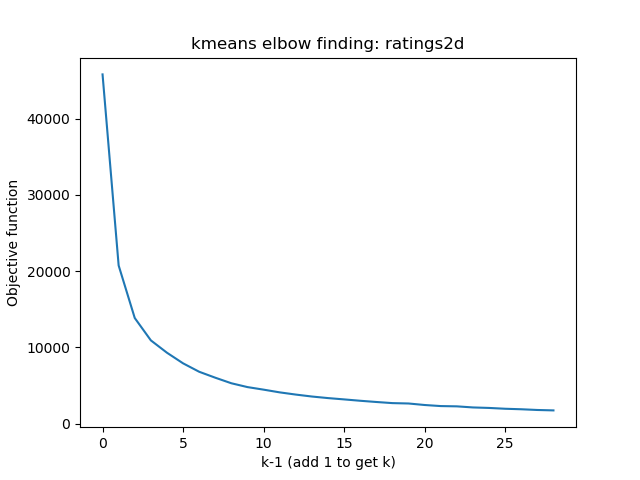
\includegraphics[width=0.9\textwidth]{kmeans_elbow_2d} % first figure itself
%         \caption{Suggests 4 clusters of users}
%     \end{minipage}\hfill
%     \begin{minipage}{0.45\textwidth}
%         \centering
%         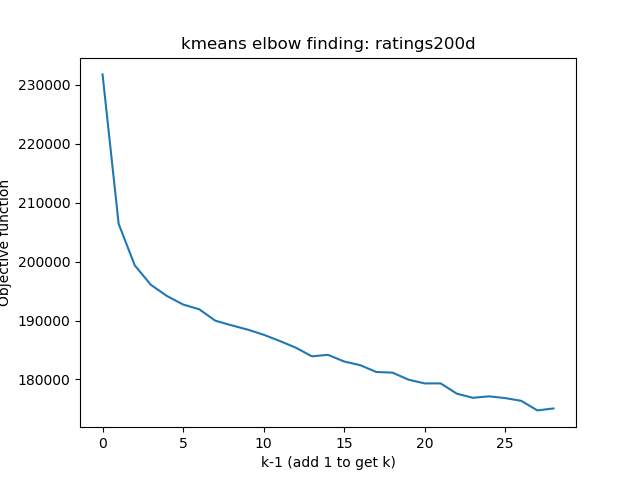
\includegraphics[width=0.9\textwidth]{kmeans_elbow_200d} % second figure itself
%         \caption{Similar results in 200d}
%     \end{minipage}
% \end{figure}

% \lstinputlisting{results/results.txt}

% \begin{figure}[h!]
%     \centering
%      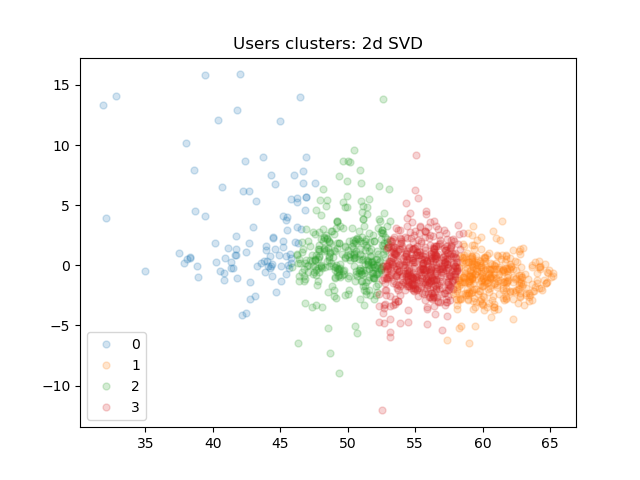
\includegraphics[width=0.5\textwidth]{user_clusters_2d}
%         \caption{Percentage of Recognition Errors}
% \end{figure}


\section{Abstract}
\textbf (100-150 words) Describe main problem statement, goal, and scope of your project.\newline

We investigate tweet sentiment over time for 400 socially connected Twitter users by dynamically visualizing changes in tweet sentiment for roughly 400,000 tweets from 2016 to present.\newline

The project scope consists of crawling the social graph, gathering tweets for each user in our graph, translating and analyzing sentiment for each tweet, and visualizing these sentiments over time. Each user is represented as a node, and the color of each node indicates that user’s sentiment at a given time. The graph is displayed using a force-directed layout. From an initial seed node, followers of a user are added along with directed edges for each $(user, follower)$ directed relationship.


\section{Introduction}
Explain motivation for the project and briefly foreshadow your report, then introduce sections.\newline

A 2015 paper by Tsugawa and Ohsaki[1] found that "negative messages are likely to be reposted more rapidly and frequently than positive and neutral messages". We did not investigate retweets but rather sought to answer whether sentiment spreads more generally between users. This could confirm and expand on the results of that paper, or simply provide some useful insight into demonstrating the folk wisdom “misery loves company”: that negative sentiment is contagious.\newline

In lieu of any substantial statistical analysis, we visualize the results on an animated graph, allowing for us to explore the data interactively and spot trends.\newline

We will begin with a general overview of the data sources and technologies used and a review of related work. Then we will discuss the specifics of our implementation, and results obtained.


\section{Background}
Describe contextual knowledge a reader would require in order to comfortably understand your project report (ex. your data sources, libraries used, technologies discussed).\newline

Twitter offers a free rate-limited API[2] which allows us to retrieve the required raw data from queries on a screen name or user id:
\begin{enumerate}
    \item \textbf{userId} : a large integer, ex. 946341920036478976 for our seed user
    \item \textbf{tweets} : most recent $\geq$ 3200 tweets for this user consisting of $[(time_1, text_1), (time_2, text_2), \dots]$ 
    \item \textbf{followers} : $[userId_1, userId_2, \dots]$
\end{enumerate}

Many of the gathered users had predominantly non-English tweets. In order to run sentiment analysis with VADER (Valence Aware Dictionary and sEntiment Reasoner)[3] we first had to translate all tweets to English. This was accomplished using Google Cloud Translate[4], a commercial service.\newline

Based on visual analysis of the data, cleaning was performed programatically. This yielded several datasets usable by the client:
\begin{enumerate}
    \item \textbf{tweets} : all tweets for all users, sorted by time $[(time, userId, sentiment, text), \dots]$
    \item \textbf{userInfo} : information for specific users such as average sentiment, number of tweets, and $followers$.
\end{enumerate}

This data was then displayed as a graph in JavaScript using the d3.js library [5]. Sentiment is then animated on each node by the timestamps of tweets. Some smoothing (rolling window averages) is selectively applied to the data to aid in spotting trends at different time granularity.


\section{Related work}
Projects with similar scope, or technologies related to the implementation of your solution. Briefly mention the projects and their relation to your report, and annotate appropriately.

\section{Methodology}
Explain implementation decisions and details. Be specific but concise, referencing information about sources when required to explain functionality. What were your goals? Why did you implement the way you did - and how did you?\newline



\section{Discussion}
This is the opportunity to showcase analysis or resulting benefits from your project implementation. Without getting into Future Work too much, briefly discuss what setbacks and desires your project implementation experience has left you with. Other than that not much advice on discussion; varies by project scope. 

\section{Future work}
Discuss possibilities of future work, for example in terms of 1) what would you consider implementing given more time on this project and 2) how can this project be used by or furthered by the open source community to improve future works?

\section{Conclusion}
Summarize the content of the report with a focus on the goal, analysis, and resulting value. Recap relevant points from the discussion, but do not restate it. Finally, you can choose to touch on future works as you close out the paper.

\appendix
\section{\\Figures and tables}

\section{\\References}
\end{document}